\documentclass{article}

\usepackage{fancyhdr}
\usepackage{extramarks}
\usepackage{amsmath}
\usepackage{minted}
\usepackage{amsthm}
\usepackage{amsfonts}
\usepackage{tikz}
\usepackage{algorithm}
\usepackage{algpseudocode}
\usepackage{adjustbox}
\usepackage{graphicx}
\usepackage{mathtools}

\usetikzlibrary{automata,positioning}
\usepackage{fullpage,enumitem,amsmath,amssymb,graphicx}
\usepackage[sort]{natbib}
\usepackage[colorlinks=true,urlcolor=blue]{hyperref}        

%
% Basic Document Settings
%

\topmargin=-0.75in
\textwidth=6.5in
\textheight=9.0in
\headsep=0.20in
\headheight = 12pt
\linespread{1.1}

\pagestyle{fancy}
\chead{\hmwkClass\ (\hmwkClassInstructor): \hmwkTitle}
\rhead{\firstxmark}
\lfoot{\lastxmark}
\cfoot{\thepage}

\renewcommand\headrulewidth{0.55pt}
\renewcommand\footrulewidth{0.55pt}

\setlength\parindent{0pt}


\setcounter{secnumdepth}{0}

%
% Homework Problem Environment
%
% This environment takes an optional argument. When given, it will adjust the
% problem counter. This is useful for when the problems given for your
% assignment aren't sequential. See the last 3 problems of this template for an
% example.

%
% Homework Details
%   - Title
%   - Due date
%   - Class
%   - Section/Time
%   - Instructor
%   - Author
%

\newcommand{\hmwkTitle}{Assignment\ \#2}
\newcommand{\hmwkDueDate}{November 19, 2021}
\newcommand{\hmwkClassCode}{COT 5405}
\newcommand{\hmwkClass}{Analysis of Algorithms}
\newcommand{\hmwkClassYear}{Fall 2021}
\newcommand{\hmwkClassInstructor}{Professor Alin Dobra}
\newcommand{\hmwkAuthorName}{\textit{Vyom Pathak}}
\newcommand{\hmwkUFID}{96703101}
\makeatletter
\setlength{\@fptop}{0pt}
\makeatother
%
%
%
% Various Helper Commands
%

% Useful for algorithms
\newcommand{\alg}[1]{\textsc{\bfseries \footnotesize #1}}

% For derivatives
\newcommand{\deriv}[1]{\frac{\mathrm{d}}{\mathrm{d}x} (#1)}

% For partial derivatives
\newcommand{\pderiv}[2]{\frac{\partial}{\partial #1} (#2)}

% Integral dx
\newcommand{\dx}{\mathrm{d}x}

% Alias for the Solution section header
\newcommand{\solution}{\textbf{\large Solution}}

% Probability commands: Expectation, Variance, Covariance, Bias
\newcommand{\E}{\mathrm{E}}
\newcommand{\Var}{\mathrm{Var}}
\newcommand{\Cov}{\mathrm{Cov}}
\newcommand{\Bias}{\mathrm{Bias}}

% norm bars
\newcommand{\norm}[1]{\left\lVert#1\right\rVert}

\begin{document}

\begin{center}
{\Large \hmwkClassCode\ \hmwkClass\ \hmwkClassYear\ \hmwkTitle}

\begin{tabular}{rl}
UFID: & \hmwkUFID \\
Name: & \hmwkAuthorName \\
Instructor: & \hmwkClassInstructor \\
Due Date: & \hmwkDueDate \\ 
% Collaborators: & [list all the people you worked with]
\end{tabular}
\end{center}

\section*{Problem 1}
\subsection*{Weighted approximate common substring [50]}
\subsubsection{Problem Definition}
Given two input strings, not necessarily of the same length, based on alphanumeric characters [A-Z], determine the best common substring. A substring is a contiguous sequence of characters within a string, and the score that determines the best substring is defined as the sum of the weights $w_l$ for each character in the sequence (i.e. $w_a$ is the weight of matching letter A) and a penalty $-\delta$ for each mismatch (negative penalty term to drive down the score). In your experiments, consider situations in which $w_l$=1 and $\delta=10$ and in which $w_l$ is proportional to the frequency of the letter in English and $\delta$ takes values between the smallest and the largest weight (multiple experiments for 10 intermediate values). Note: you are now allowed to add gaps in the solution, i.e. both matched substring have the same length. Example: inputs \lq ABCAABCAA\rq and \lq ABBCAACCBBBBBB\rq. The substring \lq CAABC\rq that starts at position 3 in the first string and position 4 in the second,  has a score 2$*w_c$+2$*w_a$-$\delta$ since the B is mismatched in the second string.
\subsubsection*{Solution}

\textbf{Algorithm} \\
\textit{Assumption:} Considering there is no gap between two characters possibles in a given string.
The algorithm can be devised as a dynamic programming problem where the bellman equation can be formed in the following way:
If the current character is matching in both the strings, add the weight of the current character to the previous best string. Otherwise, take the max of penalty  [for selecting a mismatching character] or start a new BWACS. The algorithm to find the best weighted approximate common substring is given in Algorithm~\ref{alg:wacs}.\\
\begin{algorithm}[ht]
\caption{Function for finding the best weighted approximate common sub-string}
\label{alg:wacs}
\begin{algorithmic}[1]
\State \textbf{Input:} String $A$, String $B$, penalty value $\delta$, $memo$ as a memory table with zero values.
\State \textbf{Output:} Prints the best weighted approximate common sub-string with the weight value.
\Function{FindWACS}{$A, B, \delta, memo[MAX, MAX]$}:
\State $maxWeight\leftarrow0;$
 \For {$i$ in $range(1, A.length())$}
 \For{$j$ in $range(1, B.length())$}
 \If{$A[i-1]=B[j-1]$}
 \State $memo[i,j] \leftarrow memo[i-1, j-1]+w_l;$ 
 \Else 
 \State $memo[i,j] \leftarrow max\{0, memo[i-1,j-1]-\delta\};$
 \State $maxIndex(i,j) \leftarrow i,j;$ \Comment{Store the max valued indices}
 \State $maxWeight \leftarrow max\{maxWeight, memo[i,j]\};$
 \EndIf
\EndFor
\EndFor
\State $i,j \leftarrow maxIndex(i,j);$
\State $sol \leftarrow\ '\ '$;
\While{($i>0\ and\ j>0)\ and\ (memo[i,j] > 0)$}
\State $sol \leftarrow A[i-1]+sol$;
\State $i--$;
\State $j--$;
\EndWhile
\State $print(\lq The\ Weight\ of\ the\ BWACS\ is\ :\ \rq,\ maxWeight);$
\State $print(\lq The\ BWASC\ is\ :\ \rq,\ sol);$
\EndFunction
\State $findWACS(\lq ABCC \rq,\ \lq ABCCDA\rq,\ 10,\ memo)$;
\end{algorithmic}
\end{algorithm}


\textbf{Analysis}\\\\
\textit{Proof of Correctness}\\
The algorithm always finds the best weighted approximate common substring. We prove this by claiming that the memory table is computed correctly, and then use induction.\\
\textbf{Claim:} For all $0\leq i\leq n$ and $0\leq j\leq m$, $memo[i,j] = WACS[A^i, B^j]$.\\
\textbf{Proof:} Here, base condition is that when $i=0$ and $j=0$, $memo[i,j] = 0$ which is correct. Let's assume without any loss of generality that the claim holds true for all entries $memo'[i, j]$ such that for some entry $memo[i, j]$; where $i'+j' < i+j$. Let $Sol' = WACS[A^i, B^j]$\\
If $A[i]=B[j]$, then the last character of X' must be the current character weight plus the last weight value for the $A^{i-1}$ and $B^{j-1}$. So from induction hypothesis $memo[i,j] = memo[i-1,j-1]+w_l$, we compute the entry correctly.\\
Otherwise, let x be the last character of X'. If $x\neq A[i]$, then $X'$ must be weighted approximate common substring with a penalty [$\delta$] from the previous value i.e. $A^{i-1}$, and $B^{j-1}$ or we do not extend the current solution with a penalty i.e. use 0 and start a new best weighted approximate common sub-string. Thus, it can be expressed as $WACS[A^{i}, B^{j}] = max\{memo[i-1,j-1]-\delta,0\}$, this gives the feasible  and correct solution.\\\\\\
\textit{Running Time}\\ The algorithm finds the BWACS in $O(n\cdot m)$.\\
\textbf{Proof:} Here, we loop through each character of string $A$, and for each of those character we loop through all the characters of string $B$. Thus, $n$ being the length of string $A$, and $m$ being the length of string $B$, the overall time-complexity of the solution is $O(n \cdot m)$. We store a 2-D table of length $n$ and width $m$, and thus the overall space-complexity is $O(n \cdot m)$.\\

The figure~\ref{fig:WACSrun} shows the analysis of runtime  as a function of size of the string. The evaluation is done for the same in the following way. 
\begin{enumerate}
    \item The first experiment was run on 1000 values [size of string] where the penalty was taken as -10 and the weights of each character was taken as 1.
    \item The second experiment was run on 1000. values [size of string] where the weight of each character was taken as the frequency of that character occurring in the English language~\cite{dictionaries2010frequency} and the penalty value is taken randomly between the maximum and minimum word count. 
    Also, the following figure~\ref{fig:interWACS}, 10 intermediate values shows how increasing the penalty value for the weight case; the weight of the common substring decreases as well as the size of the string decreases. The figure~\ref{fig:interWACS} shows the selection of $WACS$  for strings \lq ABCAABCAA\rq and \lq ABBCAACCBBBBBB\rq.
\end{enumerate}
\clearpage
\begin{figure}[t!]
    \centering
    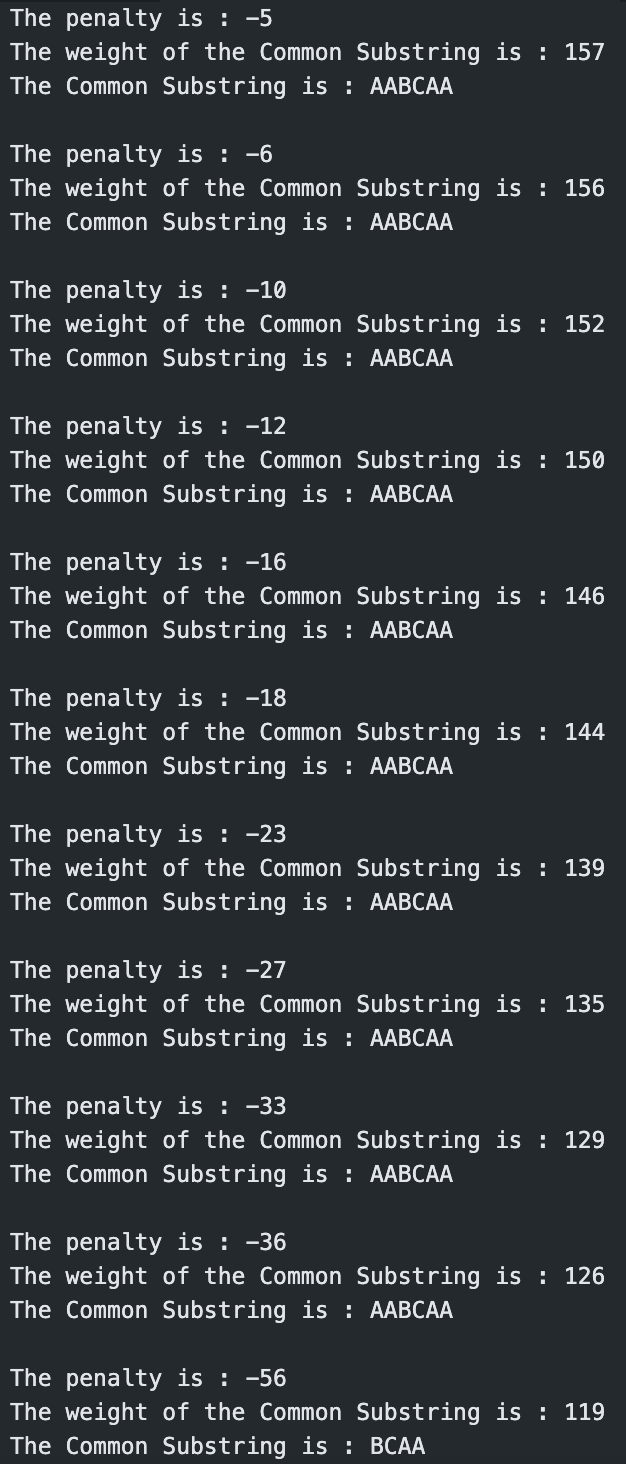
\includegraphics[width=.30\textwidth]{Screen Shot 2021-11-13 at 1.41.36 PM.png}
    \caption{Intermediate penalty value for the character frequency weight case and respective WACS}
    \label{fig:interWACS}
\end{figure}
\begin{figure}[htp]
    \centering
    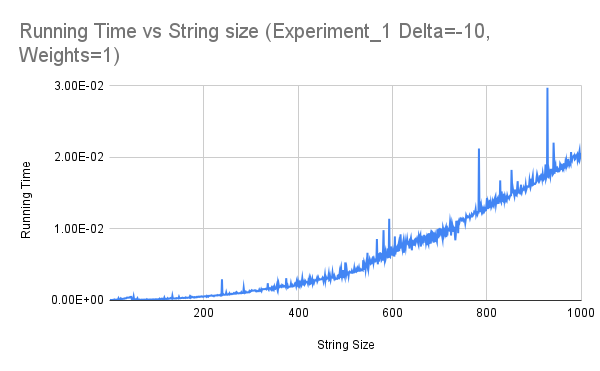
\includegraphics[width=.40\textwidth]{Running Time vs String size (Experiment_1 Delta=-10, Weights=1).png}
    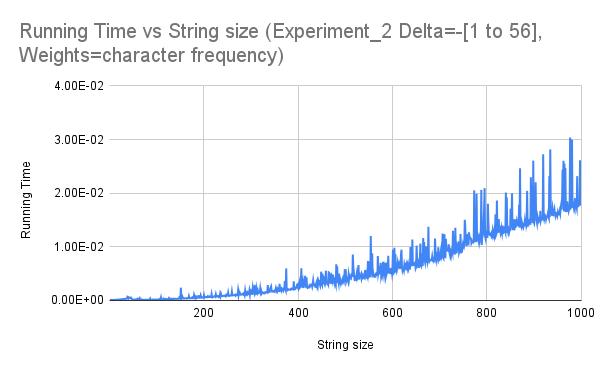
\includegraphics[width=.40\textwidth]{Running Time vs String size (Experiment_2 Delta=-[1 to 56], Weights=character frequency).png}
    \caption{Experiment 1 and 2 for checking the runtime of the WACS algorithm as a function of size of string}
    \label{fig:WACSrun}
\end{figure}
\clearpage
\section*{Problem 2}
\subsection*{Interval-based constant best approximation [50]} 
\subsubsection{Problem Definition}
Given a set of $N$ points $(x_i,y_i)$ with integer values for $x_i$ between 1 and $M$ and real values for $y_i$,  find a partitioning of the interval [1,$M$] into contiguous intervals such that the error of approximating points in each interval element by the average value of $y$ in the interval is minimized. You need to add a penalty factor proportional to the total number of intervals the solution has. For example, if you have $x \in [1,100]$ and you partition the X dimension in intervals $[1-10],[11,20],\ldots,[91,100]$ the penalty is $10*\delta$.
\subsubsection*{Solution}
\textbf{Algorithm}\\
\textit{Assumption:} For each point, the x-coordinate value is unique.
The problem is a variant of the segmented least-squared with a special value for how to control the $y$ values. Here, as the error function we consider the $y\_avg$ as the value to be used to subtract from the original $y$ value for each interval. It can be shown as follows:
\begin{align*}
    Errors[i,j] = \sum_{i=1}^{n} (y_i-y\_avg_{ij})^2\ [for\ each\ j\ from\ i\ to\ n].
\end{align*}
We calculate this effectively by using statistics i.e. sum of squares minus the square of sums which turns the above formula into the following form:
\begin{align*}
    Errors[i,j] = \frac{\sum_{k=i}^{j}x_k^2}{n} - \left(\frac{\sum_{k=i}^{j}x_k}{n} \right) ^2
\end{align*}
We can effectively pre-compute the square of sums and sum of squares in the running like cumulative sums and while calculating the errors for a range, we can find that range's sum of squares and square of sums by just subtracting by the index values for the cumulative stored in those indices. Thus, this reduces the error computation from $O(n^3)$ to $O(n^2)$. For the rest of the algorithm, the bellman equation remains the same which can be expressed as follows:
\begin{equation}
    OPT(j) = min_{1\leq i\leq j}(Errors[i,j]+delta+OPT[i-1]);
\end{equation}
Here, the problem can be understood as a linear regression model but for segments and to avoid any kind of over-fitting of too many segments we introduce the penalty which is essentially a regularization parameter. 
 The algorithm for finding interval based constant best approximation is given in Algorithm~\ref{alg:findICA}. The Algorithm~\ref{alg:calcehelp}
is a helper function which pre-computes the errors for all the points in a given range using sum of squares and square of sums optimized by a running cumulative sum.

\begin{algorithm}
\caption{Function for finding the interval-based constant best approximation}
\label{alg:findICA}
\begin{algorithmic}[1]
\State \textbf{Input:} Point Array $points$ with $x$ and $y$ coordinates, count of total number of points as $num\_points$, penalty term $delta$, Error matrix with pre-computed errors.
\State \textbf{Output:} Prints the number of segment, total cost of the solution, and prints the points between the segment indices.
\Function{findICA}{$points, num\_points,delta, Errors[MAX, MAX]$}:
\State $opt\_seg \leftarrow [\ ];$
\State $solution \leftarrow [\ ];$
\For {$j$ in $range(1, num\_points+1)$}
\State $temp\leftarrow \infty;$
\State $temp\_ind\leftarrow 0;$
 \For{$i$ in $range(1, j+1)$}
 \State $bellman\_eq\leftarrow Errors[i, j] + solution[i - 1];$
 \If{$bellman\_eq<temp$}
 \State $temp \leftarrow bellman\_eq;$ 
 \State $temp\_ind \leftarrow i;$
 \EndIf
\EndFor
\State $solution[j] \leftarrow temp + delta;$
\State $opt\_seg[j] \leftarrow temp_ind;$
\EndFor
\State $point\_indices\_stack \leftarrow \phi;$
\State $i \leftarrow num\_points;$
\State $j \leftarrow opt\_seg[num\_points];$
\While{$i>0$}
\State $point\_indices\_stack.add(i);$
\State $point\_indices\_stack.add(j);$
\State $i \leftarrow j-1;$
\State $j\leftarrow opt\_seg[i];$
\EndWhile
\State print(\lq Cost of the Optimal Solution is : \rq, $solution[num\_points]);$
\State print(\lq Total number of segments are : \rq, $point\_indices\_stack.size()/2);$
\While{$point\_indices\_stack\neq\phi$}
\State $i\_x \leftarrow point\_indices\_stack.pop();$
\State $j\_y \leftarrow point\_indices\_stack.pop();$
\State print(\lq The segments between indices: \rq, $i\_x$, \lq\ \rq, $j\_y$, \lq with error values: \rq, $Errors[i\_x,j\_y]$);
\While{$i\_x<j\_y$}
\State print(\lq( \rq, $points[i\_x-1].getX()$, \lq, \rq, $points[i\_x-1].getY()$, \lq\ )\rq);
\State $i\_x++;$
\EndWhile
\EndWhile
\EndFunction
\State $points.SortByX();$ \Comment{Sort by x-coordinate values}
\State $calculateErrors(points,num\_points);$
\State $findICA(points, num\_points,delta,Errors);$
\end{algorithmic}
\end{algorithm}

\begin{algorithm}
\caption{Helper Function to calculate the errors}
\label{alg:calcehelp}
\begin{algorithmic}[1]
\State \textbf{Input:} Point Array $points$ with $x$ and $y$ coordinates, count of total number of points as $num\_points$.
\State \textbf{Output:} Stores the Errors in a global error matrix $Errors$.
\Function{calculateERRORS}{$points, num\_points$}:
\State $prefix\_sum\_y \leftarrow [\ ];$
\State $prefix\_sum\_sqry \leftarrow [\ ];$
\For {$j$ in $range(1, num\_points+1)$}
\State $pt\leftarrow points[j-1].getY();$
\State $prefix\_sum\_y[j]\leftarrow prefix\_sum\_y[j-1]+pt;$
\State $prefix\_sum\_sqry[j] \leftarrow prefix\_sum\_sqry[j-1] +(pt\cdot pt);$
 \For{$i$ in $range(1, j+1)$}
 \If{$i=j$}
 \State $Errors[i,j] \leftarrow 0;$ 
 \Else
 \State $interval \leftarrow j-i+1;$ \Comment{Calculate the SSE error for the points between the range $i$ and $j$}
 \State $y\_sum\_ij \leftarrow prefix\_sum\_y[j] - prefix\_sum\_y[i-1];$
 \State $sqry\_sum\_ij \leftarrow prefix\_sum\_sqry[j] - prefix\_sum\_sqry[i-1];$
 \State $Errors[i, j] \leftarrow (sqry\_sum\_ij / interval) - ((y\_sum\_ij / interval) * (y\_sum
 \_ij / interval));$
 \EndIf
\EndFor
\EndFor
\EndFunction
\end{algorithmic}
\end{algorithm}

\pagebreak
\textbf{Analysis}\\
\textit{Proof of Correctness}\\
The proposed algorithm correctly computes $OPT[j]$ for each $j=1,2,3,\ldots,n$.\\
\textbf{Proof:}
\textit{Here, we assume that the FindICA is a recursive function.}
Be definition, $OPT[0]=0$. Now, taking some $j>0$, and suppose by the way of induction that the algorithm at $i$ correctly computes $OPT(k)$ for all $k<j$. Now by the induction hypothesis, we know that the algorithm $FindICA(p(j))$ will give the $OPT(p(j))$, and also the algorithm $FindICA(j-1)$ at point $j-1$ gives the solution $OPT(j-1)$ by checking every $i$ from $1 \ to\ j-1$ in equation (1). Hence, from equation (1) we are able to get the solution to $OPT(j)$ as follows:
\begin{align*}
    OPT(j) & = min_{1\leq i\leq j}(Errors[i,j]+delta+FindICA[i-1]);\\
    OPT(j) & = FindICA(j); 
\end{align*}
Hence, the proposed algorithm correctly computes $OPT[j]$ for each $j=1,2,3,\ldots,n$.
\\\\
\textit{Running Time}\\
The running time of the proposed algorithm is $O(n^2)$, where n is the number of points.\\
\textbf{Proof:} Here, first the points are sorted based on the x-coordinate values which essentially takes $O(n\cdot log(n))$ using the merge-sort algorithm. Then, the $calculateErrors()$ function runs from $1$ to number of points for the outer-loop, and for each point we run the loop with all the other points to find the interval-based error using the above mentioned formulae. We use the prefix sum calculation to efficiently calculate the sum and square of sums for each interval. Then, for finding the error is just $O(1)$. Thus, this function runs in $O(n^2)$ time.

For, the function $findICA()$, we iterate through all the points and check if the interval can be added or not based on the given bellman equation. This takes $O(n^2)$ time. After that, we print the interval coordinates from the segment indices which basically takes $O(n^2).$ Thus, the overall running time of this function is also, $O(n^2)$.

Therefore, the overall running time for all of these functions combined is $O(n^2)$.\\

The figure~\ref{fig:ICArun} shows the analysis of runtime as a function of size of the string. The analysis is done in a sense that the number of points are increased and accordingly the $y$ value and penalty ($delta$) is set. We can clearly see from the figure that the runtime of the proposed algorithm is in-fact $O(n^2)$. Also figure~\ref{fig:ICArun} shows that, for the recursive function; even if the time complexity of the algorithm is same, because of the recursive nature it takes more time than the iterative version to execute.\\

\begin{figure}[ht]
    \centering
    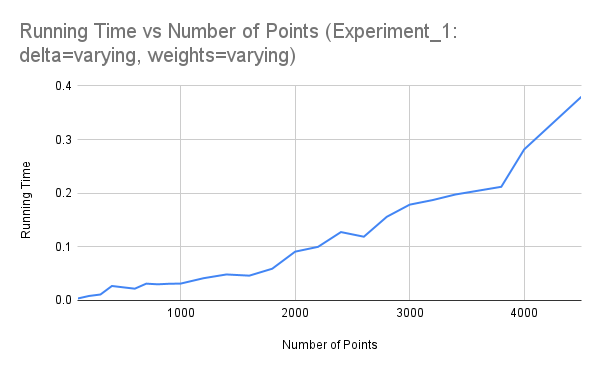
\includegraphics[width=.45\textwidth]{Running Time vs Number of Points (Experiment_1_ delta=varying, weights=varying).png}
    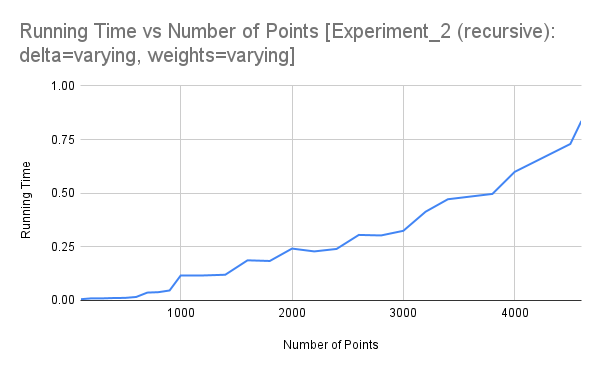
\includegraphics[width=.45\textwidth]{Running Time vs Number of Points [Experiment_2 (recursive)_ delta=varying, weights=varying].png}
    \caption{Experiment 1 for checking the runtime of the iterative ICA algorithm, and Experiment 2 as the recursive version. Both as a function of number of points}
    \label{fig:ICArun}
\end{figure}

The overall space complexity is $O(n^2)$ as we store the error matrix and the solution segments in 1-dimension.  While not using memoization, we store an 1-D array of size the number of segments which is $O(n)$. However, even after using the memoized version of the algorithm it does not budge with respect to the runtime of the algorithm i.e. the runtime of the memoized version of the algorithm is still $O(n)$ as there is no overlap in finding the segments, thus the space complexity is still more $O(n)$ in addition to the recursion stack memory. Here, the figure~\ref{fig:rec_itr} shows the analysis of space as a function of number of points for the iterative as well as the memoized version of the function $findICA()$, which clearly states that the space used in the memoized version is more because of the recursion stack $[0.94 GB > 0.88 GB]$. The memory was calculated using the \href{https://www.ej-technologies.com/products/jprofiler/overview.html}{JProfiler Tool}~\cite{cho2006jprofiler}.\\

\begin{figure}[ht]
    \centering
    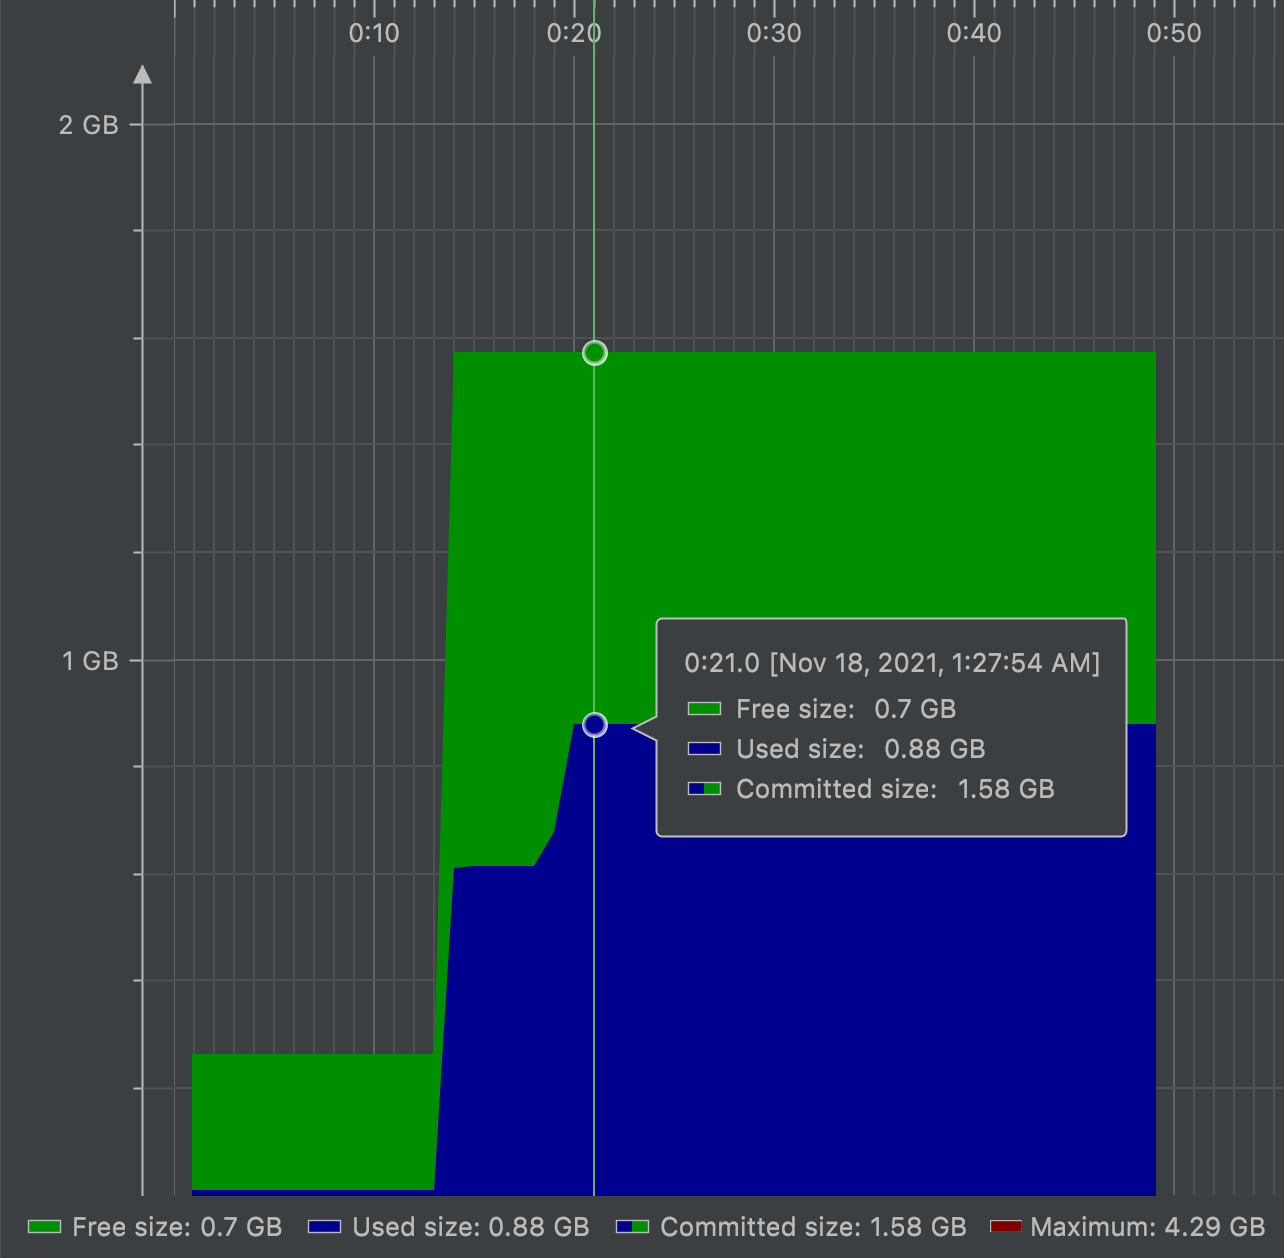
\includegraphics[width=.45\textwidth,height=.20\textheight]{Iterative.png}
    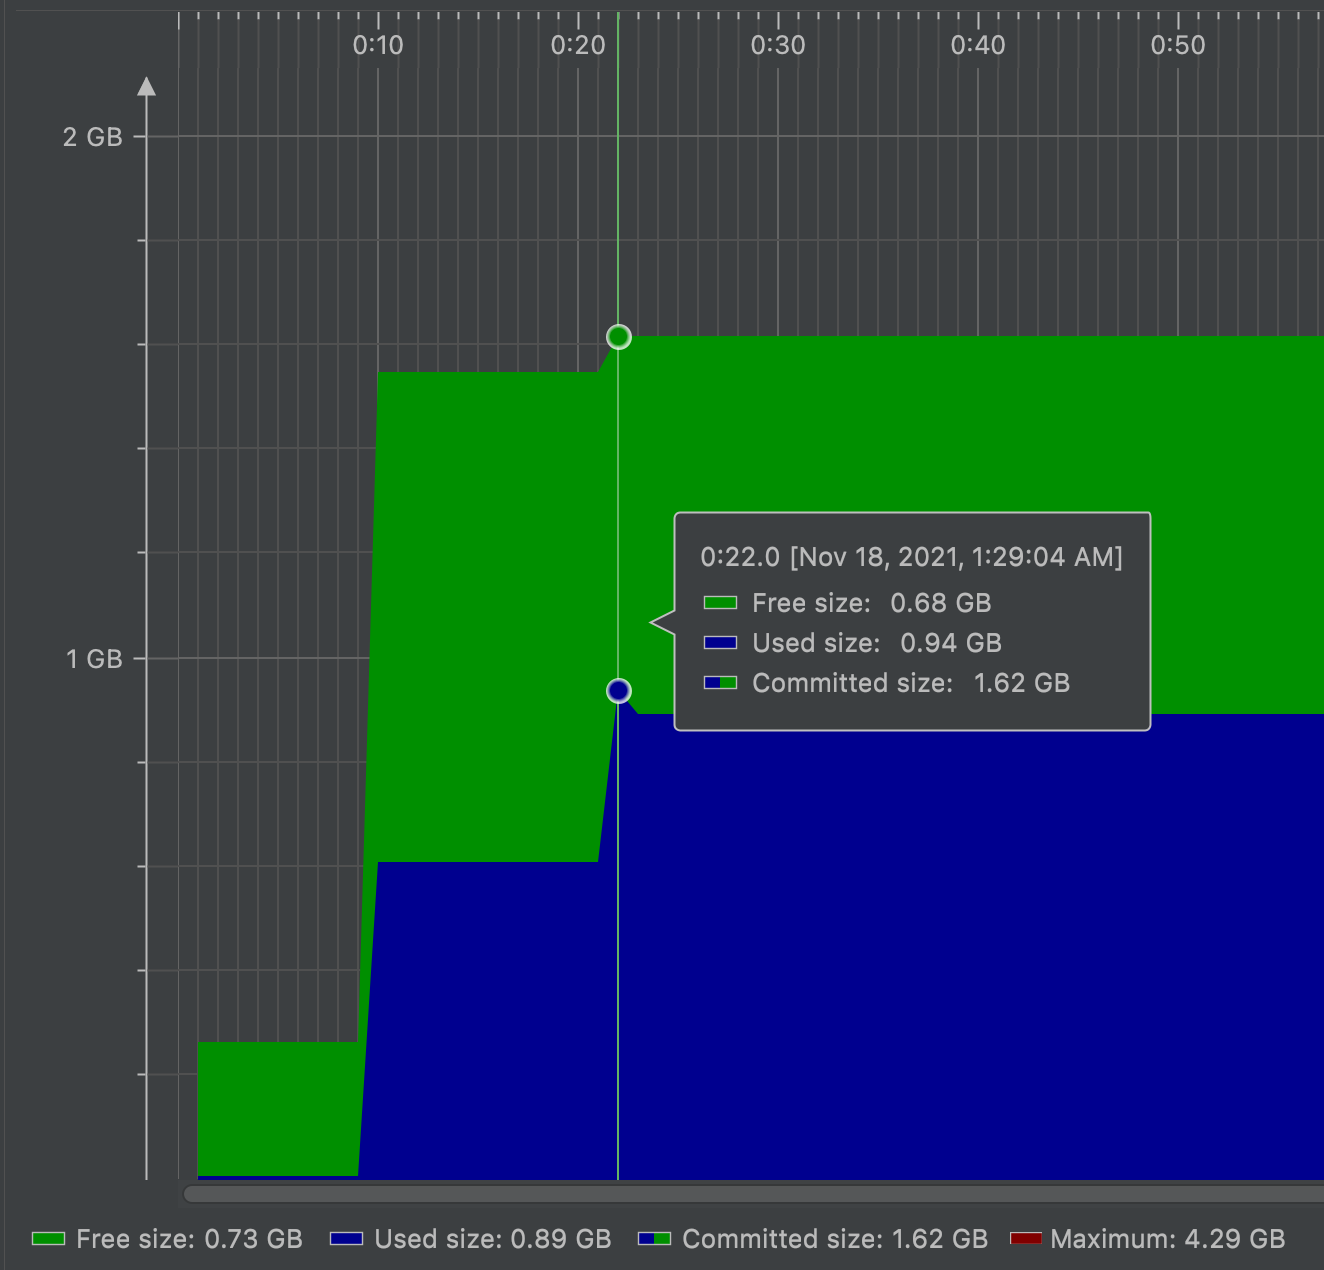
\includegraphics[width=.45\textwidth,height=.20\textheight]{Recursive.png}
    \caption{Comparision of memeory utilization for iterative [left] and memoized [right] version for the proposed algorithm}
    \label{fig:rec_itr}
\end{figure}




\clearpage
\section*{Problem 3}
\subsection*{BONUS [30]} 
\subsubsection*{Problem Definition}
Generalize problem 2 to a 2D grid for the input, i.e. the input is of the form $x_i,y_i,z_i$ with $x_i,y_i\in[1..M]$ and $z_i$ a real number. You must both develop the theory and implement this version of the algorithm and test it similarly to the setup above.
\subsubsection*{Solution}
The proposed problem essentially cannot be generalized from the previous 2D case because no-optimal sub-structure can be found to solve the given problem using Dynamic-Programming in polynomial time.\\
\textbf{Proof: } 

Proof by counter-example. Here, let's assume that somehow the previous algorithm for the 2D case works for the 3D case with a modification in the the selection of point accordingly. Now, consider the following 3D case points: (1, 2, 3.0), (2, 2, 4.0), (3, 4, 5.0), (1,4,10.0), (3,5,1.0), (3,3,2.0), and the delta value as $10.0$. Now, even with the modifications to the 2D algorithms, we can sort the points first on $x$ values and then on $y$ values which is essentially $O(n\cdot log(n))$. After that, we calculate the Errors similar to 2D case but in a 3D manner which turns the runtime algorithm to $O(n^3)$. Further, to find the optimal cost, the problem is that it is in 3D space. Thus even the modified version of the previous problem cannot be used because the equation (1) is true for 2D case but for the 3D case it doesn't work in a simple linear way as we have measure the change in points in 2 dimension which cannot be executed in polynomial time with an optimal sub-structure.
\section*{Guide to Code}
Both the codes were written in Java language. 
\subsubsection*{Steps}
\begin{enumerate}
    \item Download and Install JDK 11+ on your system using the following link:~\href{https://www.oracle.com/java/technologies/downloads/}{JDK}
    \item Create new java projects one-by-one and use the $WACS.java$ and $ICA.java$ for prob. 1 and prob. 2.
    \item Run the java projects and interactively give input according to the prompt.
\end{enumerate}
\textit{$^*$Tip: Use VS code and Java extensions for easy install and execution.}\\
\markright{}
\bibliographystyle{plain}
\bibliography{main}
\end{document}
